\section{PCA on llama3 and mistral}
\label{app:sec:pca}

To investigate if the singular components that have the highest singular values are able to capture most of the information of a weight matrix, we conducted Principle Component Analysis (PCA) on the weight matrices in \llama and \mistral (see Figures~\ref{fig:pca_analysis_llama3_8b} and~\ref{fig:pca_analysis_mistral_7b}).
In each figure, we plot the variance that is captured by the top $r$ components across all the layers in each type of modules for a weight matrix $W \in \mathbb{R}^{m \times n}$:
$$\text{ratio} = \frac{\sum_{i=1}^r \sigma_i}{\sum_{j=1}^{\min(m, n)} \sigma_j}$$
Here, $\sigma$'s are the ordered (from largest to smallest) singular values on the weight matrix $W$.
It is easy to see from the figures that when $r=256$, less than 50\% of the variance is captured by these top components on average.
For the MLP layers, this fraction is even lower than 20\%.
On the other hand, the ranks adopted by LoRA-XS or similar methods are much less than 256, resulting in even more information loss and restrictions in their modeling power that relies mostly on these $r$ components.


\begin{figure}[!h]
    \centering
    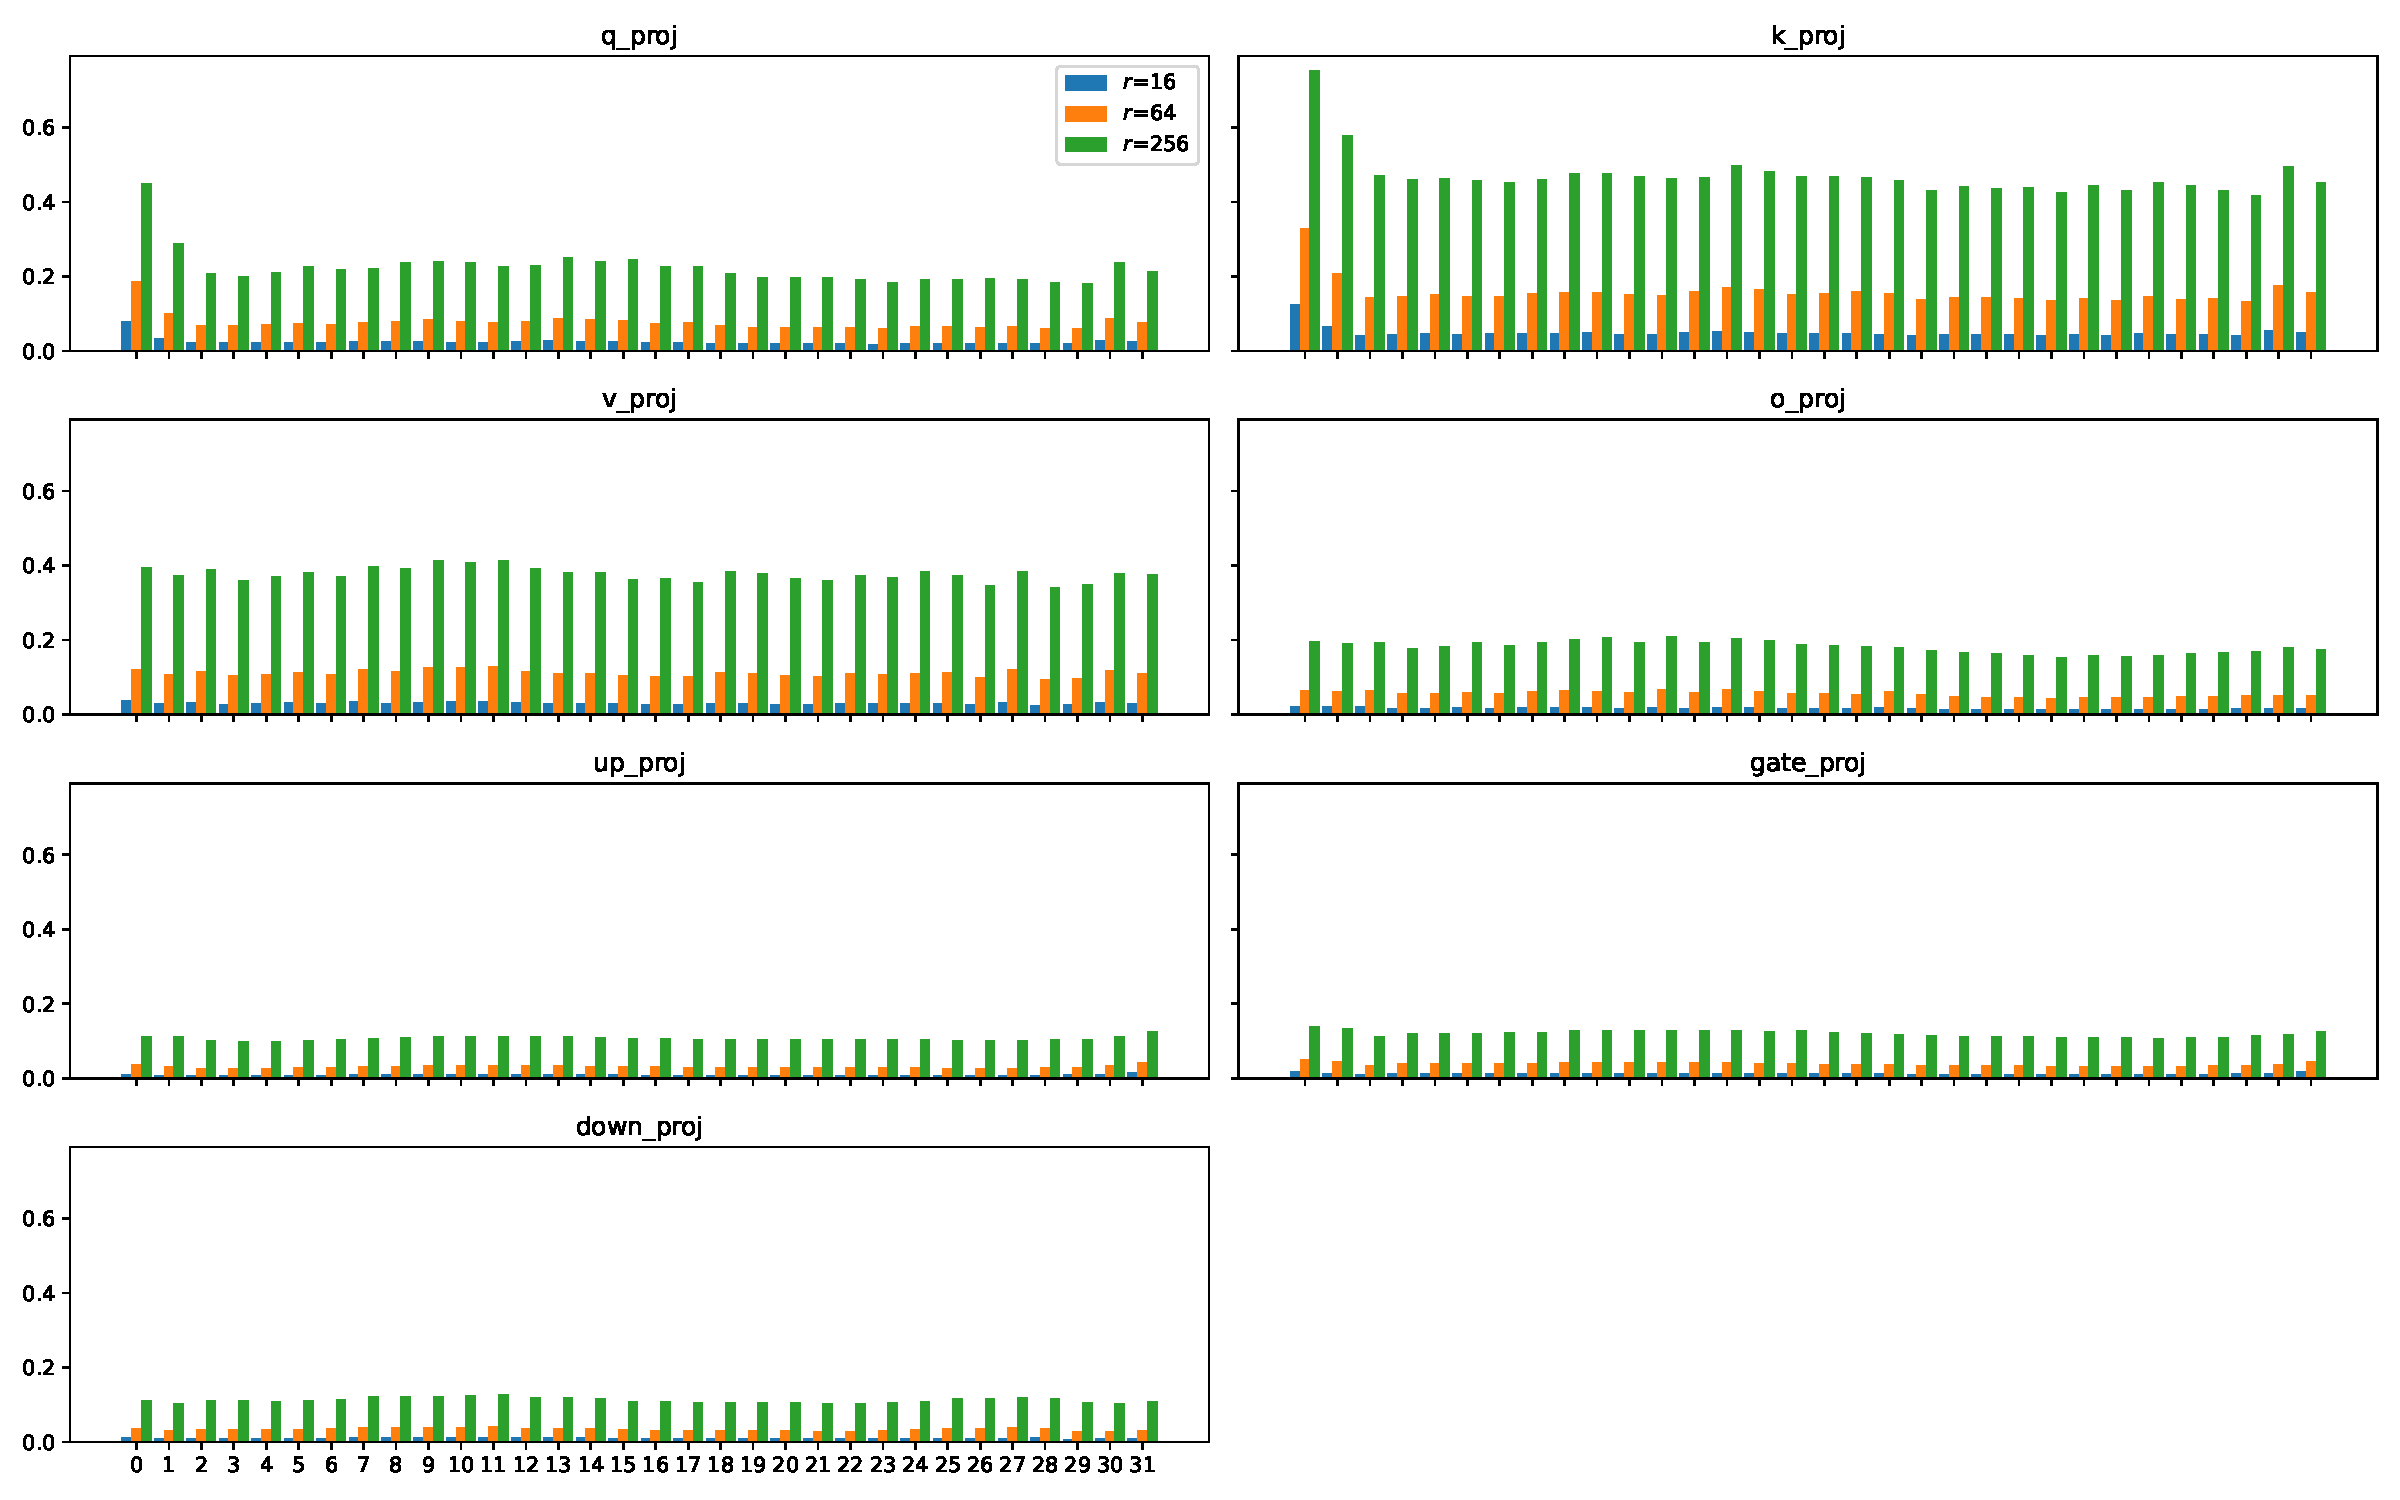
\includegraphics[width=\textwidth]{images/pca_analysis_llama3-8b.pdf}
    \vspace{-6mm}
    \caption{\textbf{PCA of \llama.} We show the ratio of the variance captured by the top $r$ singular components on the y-axis, and the layer indices on the x-axis. Except for the Query, Key and Value projection matrices, small $r$ values only capture a tiny fraction of variance in singular values in the parameter matrices.}
    \vspace{-4mm}
    \label{fig:pca_analysis_llama3_8b}
\end{figure}


\begin{figure}[!h]
    \centering
    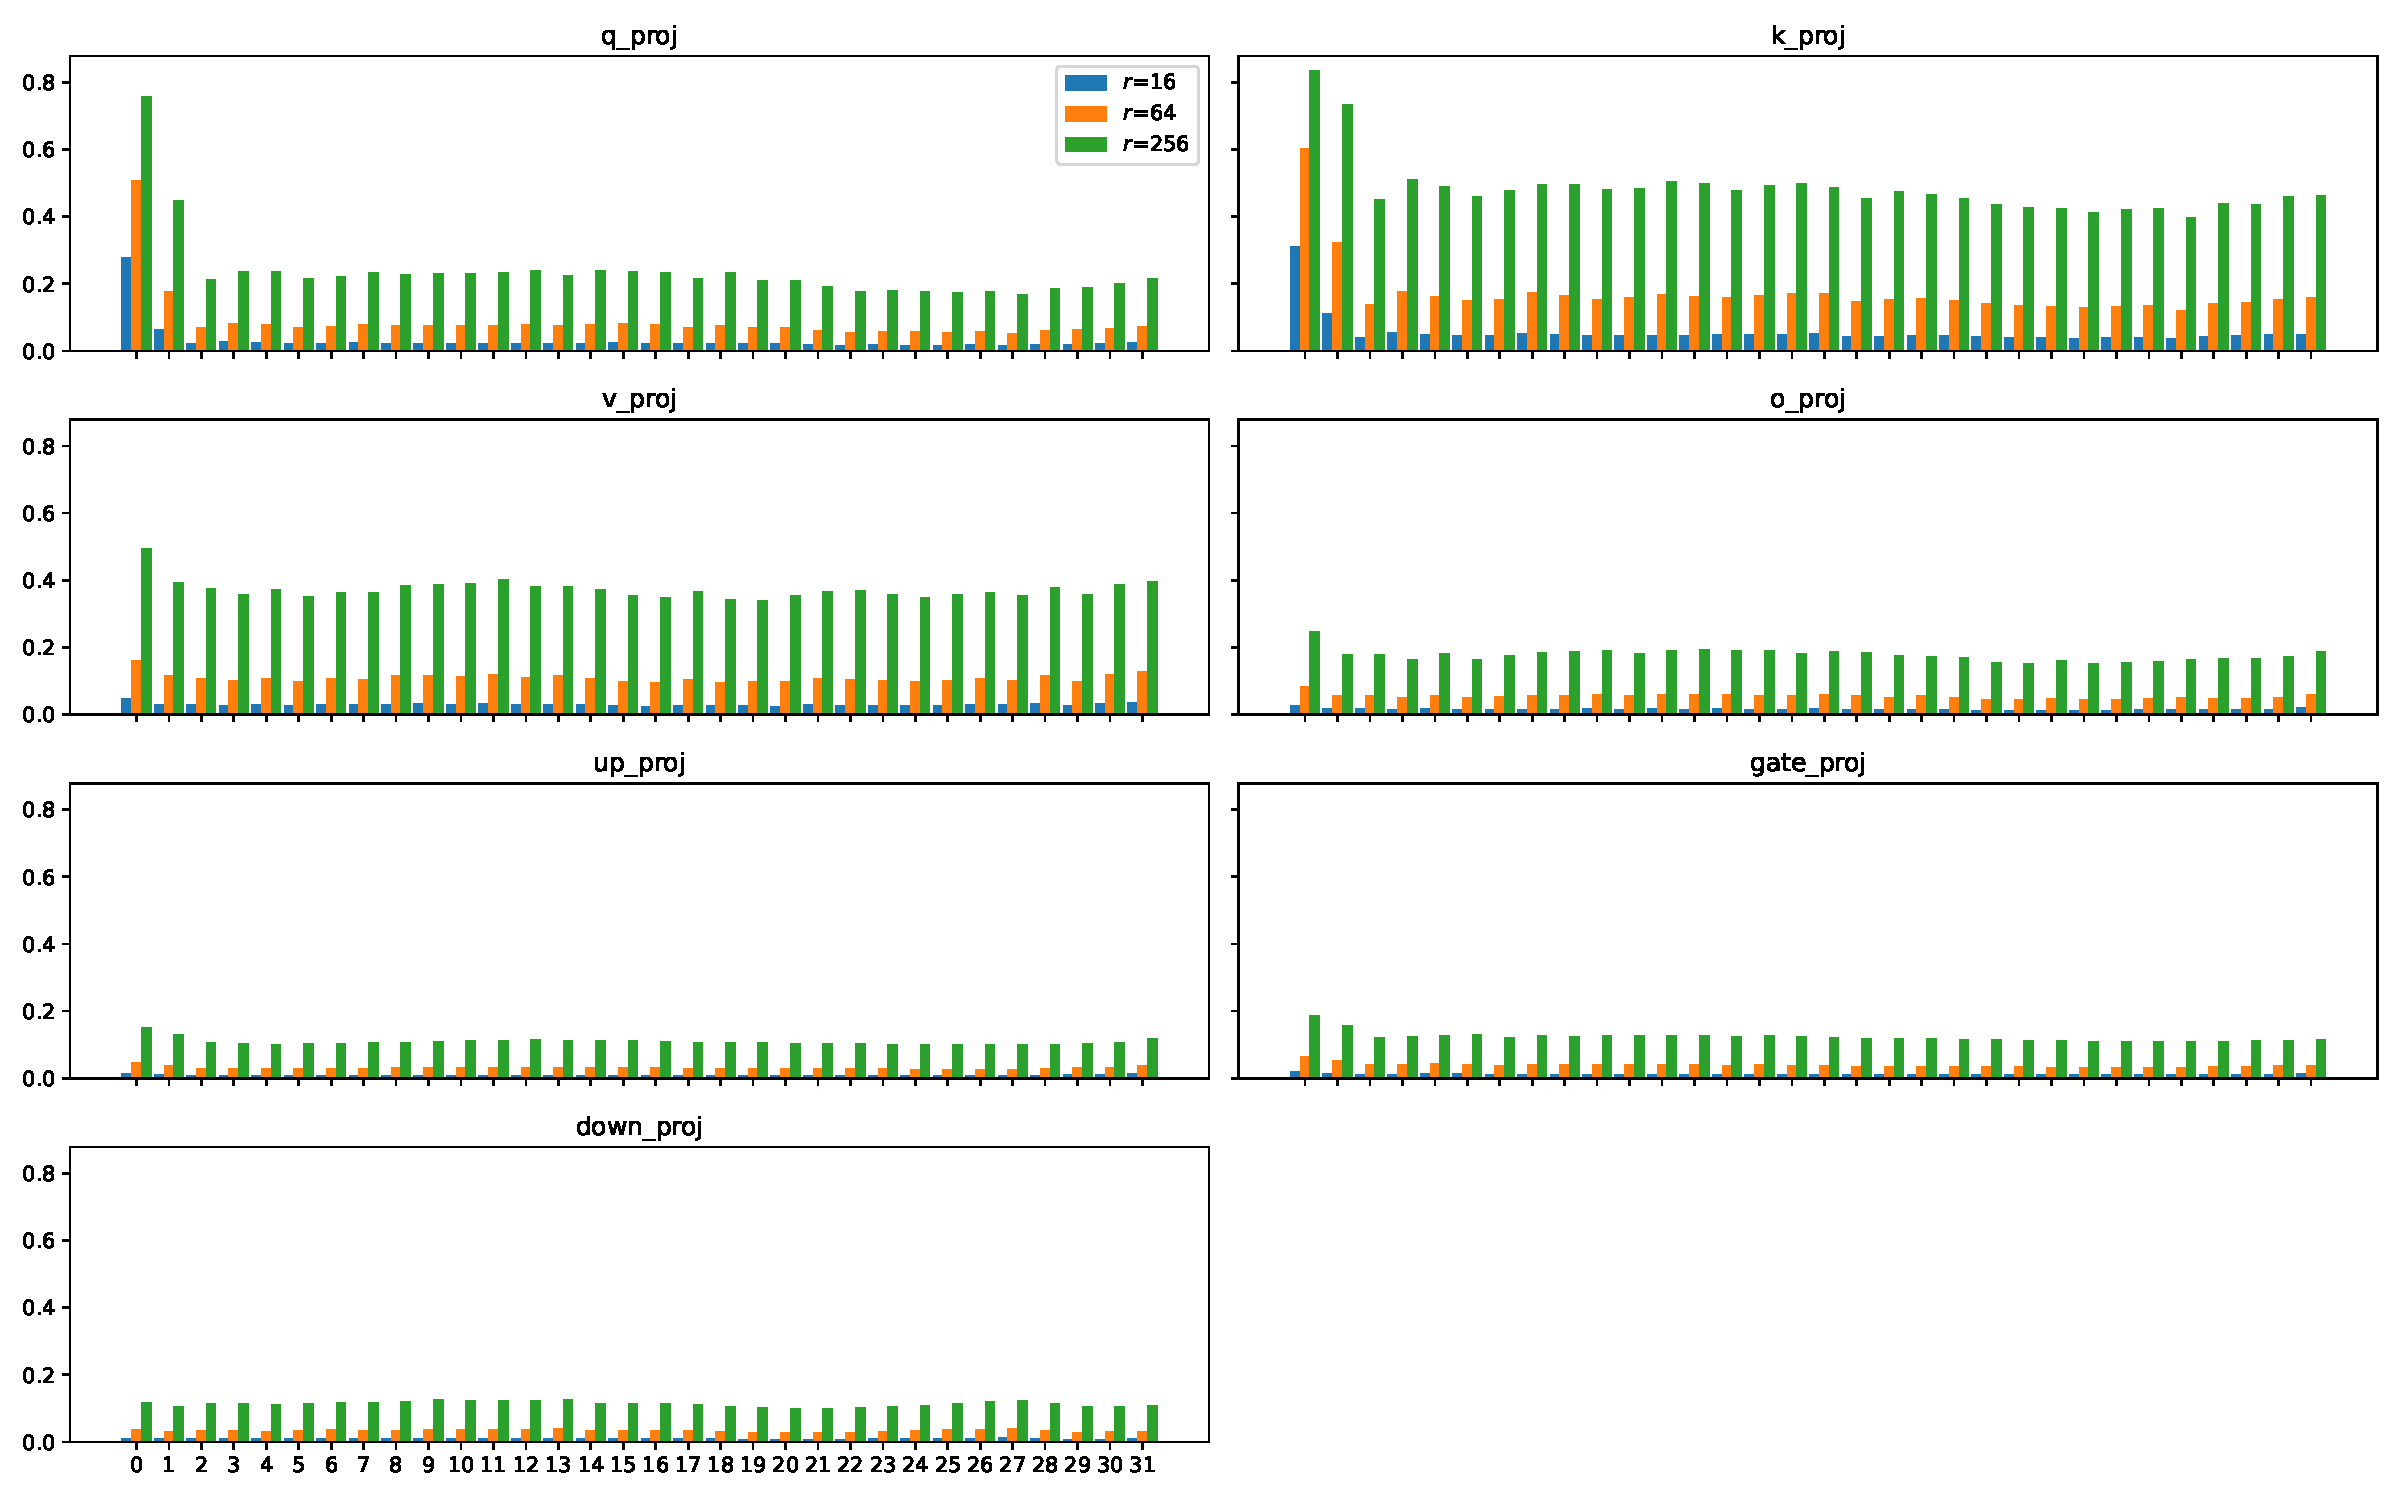
\includegraphics[width=\textwidth]{images/pca_analysis_mistral-7b.pdf}
    \vspace{-6mm}
    \caption{\textbf{PCA of \mistral.} We show the ratio of the variance captured by the top $r$ singular components on the y-axis, and the layer indices on the x-axis. Except for the Query, Key and Value projection matrices, small $r$ values only capture a tiny fraction of variance in singular values in the parameter matrices.}
    \vspace{-4mm}
    \label{fig:pca_analysis_mistral_7b}
\end{figure}